\documentclass{article}

%%%%%%%%%%%%%%%%%%%%%%%%%
% Packages & Macros
%%%%%%%%%%%%%%%%%%%%%%%%%

% For including graphics
\usepackage{graphicx}

% For title page
\usepackage{datetime}
\newdateformat{monthyeardate}{\monthname[\THEMONTH] \THEYEAR}

% For supporting linking
\usepackage{hyperref}
\hypersetup{colorlinks,urlcolor=blue,linkcolor=blue}

% For table colouring (in command line tables)
\usepackage{colortbl}

% For supporting footnotes in tables
\usepackage{footnote} 
\makesavenoteenv{tabular}

% For centering multi-line captions
\usepackage[justification=centering]{caption}

% For string comparison in macros
\usepackage{etoolbox} 

%%%%%%%%%%%%%%%%%%%%%%%%%
% Tool-Specific Macros
%%%%%%%%%%%%%%%%%%%%%%%%%
\usepackage{xspace}

\newcommand{\args}[1] {\textit{#1}}
\newcommand{\cmd}[1] {\texttt{#1}}     % Use for command window commands, e.g., \cmd{svn up}
\newcommand{\block}[1] {\textsf{#1}}   % Use for Simulink block names, e.g., \cmd{Subsystem1}
\newcommand{\signal}[1] {\textsf{#1}}   % Use for Simulink block names, e.g., \cmd{Subsystem1}
\newcommand{\ring}[1] {\textsf{#1}} 	 % Use for files names and paths
\newcommand{\keyword}[1] {\texttt{#1}} % Use for keywords of programming languages, e.g., \keyword{while}
\newcommand{\file}[1] {\texttt{#1}} 	 % Use for files names and paths
\newcommand{\param}[1] {\textsf{#1}}   % Use for block parameter names, e.g., \param{BlockType}

% Matlab Products
\newcommand{\matlab}{\textsc{Matlab}\@\xspace}
\newcommand{\Matlab}{\textsc{Matlab}\@\xspace}
\newcommand{\Simulink}{Simulink\@\xspace}
\newcommand{\simulink}{Simulink\@\xspace}
\newcommand{\SDV}{Simulink Design Verifier\@\xspace}
\newcommand{\mpath}{\Matlab search path\@\xspace}

% Block Names (not BlockType)
\newcommand{\ds}{\block{Data Store}\@\xspace}
\newcommand{\DSM}{\block{Data Store Memory}\@\xspace}
\newcommand{\DSR}{\block{Data Store Read}\@\xspace}
\newcommand{\DSW}{\block{Data Store Write}\@\xspace}
\newcommand{\DSRW}{\block{Data Store Read/Write}\@\xspace}
\newcommand{\DSMRW}{\block{Data Store Memory/Read/Write}\@\xspace}

\newcommand{\goto}{\block{Goto}\@\xspace}
\newcommand{\from}{\block{From}\@\xspace}

\newcommand{\inport}{\block{Inport}\@\xspace}
\newcommand{\outport}{\block{Outport}\@\xspace}
\newcommand{\constant}{\block{Constant}\@\xspace}
\newcommand{\ground}{\block{Ground}\@\xspace}
\newcommand{\subsystem}{\block{Subsystem}\@\xspace}

\newcommand{\logic}{\block{Logical Operator}\@\xspace}
\newcommand{\relational}{\block{Relational Operator}\@\xspace}
\newcommand{\ifblk}{\block{If}\@\xspace}
\newcommand{\switch}{\block{Switch}\@\xspace}
\newcommand{\merge}{\block{Merge}\@\xspace}

\newcommand{\docblock}{\block{DocBlock}\@\xspace}

\newcommand{\simfunc}{\block{Simulink Function}\@\xspace}
\newcommand{\simfunccaller}{\block{Function Caller}\@\xspace}

\newcommand{\toworkspace}{\block{To Workspace}\@\xspace}
\newcommand{\fromworkspace}{\block{From Workspace}\@\xspace}

\newcommand{\tofile}{\block{To File}\@\xspace}
\newcommand{\fromfile}{\block{From File}\@\xspace}

\newcommand{\fromspreadsheet}{\block{From Spreadsheet}\@\xspace}

\newcommand{\modelref}{\block{Model Reference}\@\xspace}
\newcommand{\library}{\block{Library}\@\xspace}
\newcommand{\librarylink}{\block{Library Link}\@\xspace}

% Commonly used parameters
\newcommand{\AND}{\param{AND}\@\xspace}
\newcommand{\OR}{\param{OR}\@\xspace}
\newcommand{\NOT}{\param{NOT}\@\xspace}
\newcommand{\NOR}{\param{NOR}\@\xspace}
\newcommand{\NAND}{\param{NAND}\@\xspace}
\newcommand{\XOR}{\param{XOR}\@\xspace}
\newcommand{\NXOR}{\param{NXOR}\@\xspace}

% Common Abbreviations
% Example
\newcommand{\eg}{\textrm{e.g.,}\@\xspace}

% That Is To Say
\newcommand{\ie}{\textrm{i.e.,}\@\xspace}

% And So On
\newcommand{\etc}{\textrm{etc.}\@\xspace}

% And Others
\newcommand{\etal}{\textrm{et al.}\@\xspace}

% With Respect To
\newcommand{\wrt}{\textrm{w.r.t.}\@\xspace}

% Vice Versa
\newcommand{\vrsa}{\textrm{vice versa}\@\xspace}

% Symbols
\usepackage{amssymb}
\newcommand{\checkbox}{\makebox[0pt][l]{$\square$}\raisebox{.15ex}{\hspace{0.1em}$\checkmark$}}%
\newcommand{\uncheckbox}{$\square$~}%


\newcommand{\ToolName}{Line-Goto/From Tool\@\xspace}

\newcommand{\menu}[2]{%
	\ifthenelse{\equal{#1}{1}}{Goto/Froms to Line}{}%
  	\ifthenelse{\equal{#1}{2}}{Line to Goto/Froms}{}%
}

\newcommand{\func}[2]{%
	\ifthenelse{\equal{#1}{1}}{\cmd{goto2Line}}{}%
  	\ifthenelse{\equal{#1}{2}}{\cmd{line2Goto}}{}%
}

\newcommand{\toolFolder}{\cmd{LineToGotoFrom}}
\newcommand{\demoName}{\cmd{Line2GotoFromDemo}\@\xspace}

%%%%%%%%%%%%%%%%%%%%%%%%%
% Document
%%%%%%%%%%%%%%%%%%%%%%%%%

\begin{document}

%%%%%%%%%%%%%%%%%%%%%%%%%%%%%%%%%%%%%%%%%%%%%%%%%%%%%%%%%%%%%%%%%%%
% Title Page
%%%%%%%%%%%%%%%%%%%%%%%%%%%%%%%%%%%%%%%%%%%%%%%%%%%%%%%%%%%%%%%%%%%
\title{\ToolName}
\date{\monthyeardate\today}
\maketitle
\vfill

\begin{figure}
	\centering
	
\includegraphics[]{../figs/McSCert_Logo.pdf} \\
	McMaster Centre for Software Certification (McSCert)
\end{figure}

\newpage

%%%%%%%%%%%%%%%%%%%%%%%%%%%%%%%%%%%%%%%%%%%%%%%%%%%%%%%%%%%%%%%%%%%
% Table of Contents
%%%%%%%%%%%%%%%%%%%%%%%%%%%%%%%%%%%%%%%%%%%%%%%%%%%%%%%%%%%%%%%%%%%

\tableofcontents
\newpage

%%%%%%%%%%%%%%%%%%%%%%%%%%%%%%%%%%%%%%%%%%%%%%%%%%%%%%%%%%%%%%%%%%%
% Introduction
%%%%%%%%%%%%%%%%%%%%%%%%%%%%%%%%%%%%%%%%%%%%%%%%%%%%%%%%%%%%%%%%%%%
\section{Introduction}

% Briefly, what is the tool?
% Provide any background or references.
The \ToolName is used in \Matlab/\Simulink to convert signal lines to \goto/\from blocks, as well as \goto/\from blocks to signal lines. 
% Why is it useful?
The tool aims to facilitate software development activities in \Matlab \Simulink by automating frequently performed actions by developers when creating, modifying, or maintaining models. The use of \goto/\from blocks or signal lines helps to increase readability where appropriate. In models with many signal line crossings, converting some signal lines to \goto/\from blocks will help in decluttering the model. Conversely, using signal lines for straightforward connections, instead of \goto/\from blocks, will allow developers to more easily  follow the visual data flow.

% Is there more information?
%\subsection*{More Information}
%For more information about ..., an interested reader is referred to:
%
%\vspace{1em}
% <citation goes here>
	
%%%%%%%%%%%%%%%%%%%%%%%%%%%%%%%%%%%%%%%%%%%%%%%%%%%%%%%%%%%%%%%%%%%
% How to Use the Tool
%%%%%%%%%%%%%%%%%%%%%%%%%%%%%%%%%%%%%%%%%%%%%%%%%%%%%%%%%%%%%%%%%%%
\section{How to Use the Tool}
This section describes what must be done to setup the \ToolName, as well as how to use the tool.

%--------------------------------------- 
% What needs to be done before the tool can be used? 
% What needs to be done to a model in order for it to work with the tool?
%---------------------------------------
\subsection{Prerequisites and Installation}

\begin{enumerate}
  \item Use \Matlab/\Simulink 2011b or newer.
	\item To install the tool,
	\begin{enumerate}
		\item from a \file{.zip} file --- unzip the contents into your desired location. Ensure the unzipped folder and subfolders are present in your \mpath, or add them if they are not present. Run \href{https://www.mathworks.com/help/simulink/ug/registering-customizations.html}{sl\_refresh\_customizations} to refresh the Context Menu. 
		\item from a \file{.mltbx} file --- simply open \Matlab and double-click on the file. Your \mpath should be automatically configured.
		\item from the files only --- add the folders and subfolders to your \mpath. Run \href{https://www.mathworks.com/help/simulink/ug/registering-customizations.html}{sl\_refresh\_customizations} to refresh the Context Menu.
	\end{enumerate}
	\begin{itemize}
		\item \textit{Note:} If running the command ``\cmd{which line2Goto}'' indicates that the script is not found, then the tool needs to be added to the \mpath.
		For information on adding files to the \mpath, please see the \href{https://www.mathworks.com/help/matlab/matlab_env/add-remove-or-reorder-folders-on-the-search-path.html}{MathWorks documentation}.
	\end{itemize}
	\item Ensure the Simulink-Utility folder is on your \mpath. This is a dependency for the tool to work correctly.
	\item Ensure your model is open and unlocked.
\end{enumerate}

%---------------------------------------
% How/when do you access the tool?
%---------------------------------------
\subsection{Getting Started}
The tool can be used via the \Simulink Context Menu, which can be viewed by right-clicking in a model. The following options can be available, depending on what is selected in the model. These options are listed below and shown in Figure~\ref{FIG:contextMenu}.
\begin{itemize}
	\item \emph{\menu{1}} -- Available when one or more \goto/\from blocks are selected.
	\item \emph{\menu{2}} -- Available when one or more signal lines are selected.
\end{itemize}

\begin{figure}
	\centering
	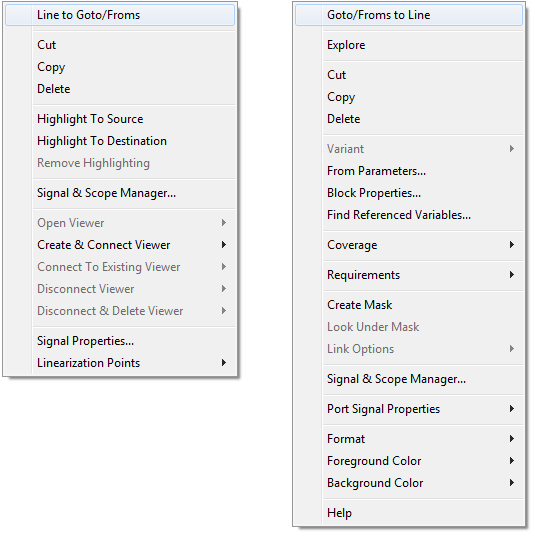
\includegraphics[width=0.7\textwidth]{../figs/ContextMenu}
	\caption{How the tool will appear in the \Simulink Context Menu.}
	\label{FIG:contextMenu}
\end{figure}

%---------------------------------------
% What are the main uses of the tool?
%---------------------------------------
\newpage
\subsection{Functionality}
This section describes the tool functionality when being used from the \Simulink Context Menu (Figure~\ref{FIG:contextMenu}).

\subsubsection*{\menu{1}}
Selecting one or more \goto/\from blocks and then selecting \cmd{\menu{1}} from the Context Menu will convert the selected blocks to signal line connections. 
Multiple blocks can be selected by either dragging the cursor over several blocks, or by pressing \cmd{shift} and then selecting blocks.

\goto/\from blocks with global or scoped visibilities, i.e., those with corresponding blocks outside of the current subsystem, will not be converted.

\subsubsection*{\menu{2}}
Selecting one or more signal lines and then selecting \cmd{\menu{2}} from the Context Menu will convert the selected signal lines to \goto/\from connections. If a signal line has a name which is a valid variable name, it will automatically be used as the \goto/\from tag. If the line has no name or it is an invalid variable name, the propagated signal name will be used as the tag. If propagation is off or the propagated signal name is not valid, the user will be prompted to provide a tag name through the GUI shown in Figure~\ref{FIG:prompt_name}. If the tag name entered is not a valid variable name, the user will be prompted to provide another name. If the tag corresponds to existing \goto/\from blocks which are within scope, that is, they will conflict, the user will be prompted to provide another name.

\begin{figure}
	\centering
	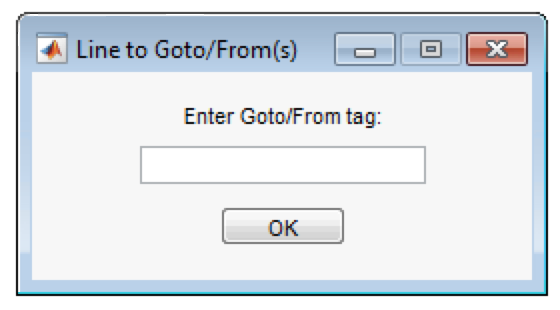
\includegraphics[width=0.5\textwidth]{../figs/Prompt_Name}
	\caption{Tool dialog window prompting for a \goto/\from tag.}
	\label{FIG:prompt_name}
\end{figure}

This operation can be done on multiple signal lines at a time. To do so, multiple lines can be selected by either dragging the cursor over several signal lines, or by pressing shift and then selecting the desired signal lines.

\textit{\textbf{Note:} For \Matlab 2011b \Simulink, it is not possible to directly right-click on multiple signal lines. To overcome this, you must also select one of the source blocks of a selected signal line, and perform the right-click on this block.}

%---------------------------------------
% What are the configuration options for the tool?
%---------------------------------------
\subsection{Configuration Parameters}
The configuration file \cmd{config.txt} is included in \cmd{\toolFolder\textbackslash src}. The following configuration parameters are utilized by the tool, and can be modified by the user in order to tailor tool functionality:

\begin{itemize}
	\item \cmd{resize\_block} --- Enables or disables the the resizing of \goto/\from block length to a specific size.
	\item \cmd{static\_resize} --- Enables or disables the ability to resize \goto/\from block length to a fixed value. Otherwise, \goto/\from blocks will be resized dynamically. This parameter is used only when \cmd{resize\_block} is enabled.
	\item \cmd{static\_length} --- The number of pixels that \goto/\from blocks are resized to lengthwise, when \cmd{static\_resize} is enabled.
	\item \cmd{px\_per\_letter} --- The number of pixels to allocate per letter of a \goto/\from
tag, that the block will be resized to. This parameter is used when \cmd{static\_length} is disabled (i.e., dynamic resizing is enabled).
	\item \cmd{block\_offset} --- The distance in pixels between \goto/\from blocks and the blocks that they are connected to.
	\item \cmd{line\_routing} --- Enables or disables \emph{autorouting} when adding new lines. 
	\item \cmd{from\_signal\_naming} --- Enables or disables the naming of signals out of the new \from block(s) to match the signal name going into the \goto block.
	\item \cmd{from\_signal\_propagation} --- Enables or disables the propagation of signals through the new \from block(s).
\end{itemize}

Please see the configuration file for more details regarding parameter usage and accepted values. These parameters can be modified with \Matlab open, and do not require that \Matlab be restarted for the changes to take effect.

%---------------------------------------
% What else does the tool do?
%---------------------------------------
\subsection{Errors and Warnings}
Any errors or warnings during tool use will be visible in the \Matlab Command Window.

%%%%%%%%%%%%%%%%%%%%%%%%%%%%%%%%%%%%%%%%%%%%%%%%%%%%%%%%%%%%%%%%%%%
% Example
%%%%%%%%%%%%%%%%%%%%%%%%%%%%%%%%%%%%%%%%%%%%%%%%%%%%%%%%%%%%%%%%%%%
\section{Example}

Use the command \demoName in the \Simulink Command Window to open the example model, shown in Figure~\ref{FIG:demo1}. There are \goto/\from blocks in this example with tag \block{A}. To transform them into a signal line connection, right-click on the \goto block, one of the \from blocks, or by selecting all these blocks. Then choose the \cmd{\menu{1}} option from the Context Menu. The resulting model is given in Figure~\ref{FIG:demo2}. Likewise, to transform the line named \keyword{signalB} to a \goto/\from block connection, right-click on the signal line and select the \cmd{\menu{2}} option. The resulting model is given in Figure~\ref{FIG:demo3}.

\begin{figure}
	\centering
	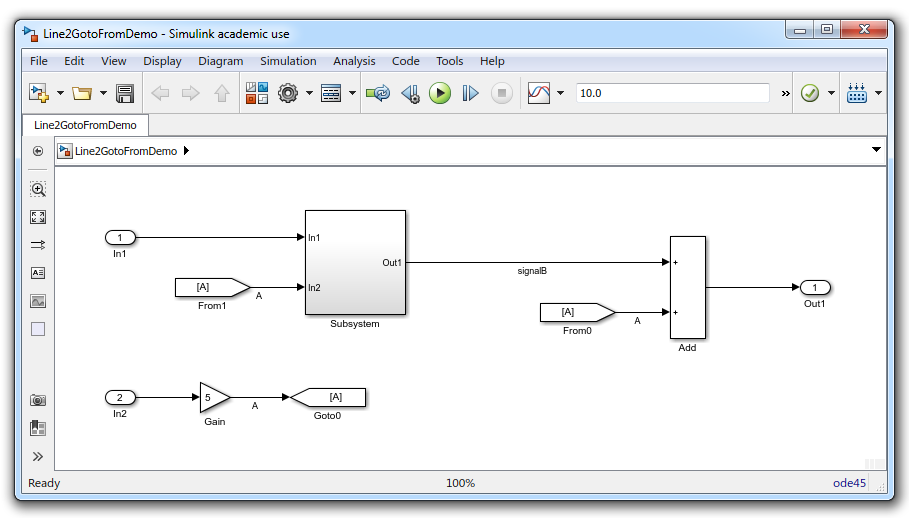
\includegraphics[width=\textwidth]{../figs/Demo1}
	\caption{\ToolName demo model.}
	\label{FIG:demo1}
\end{figure}

\begin{figure}
	\centering
	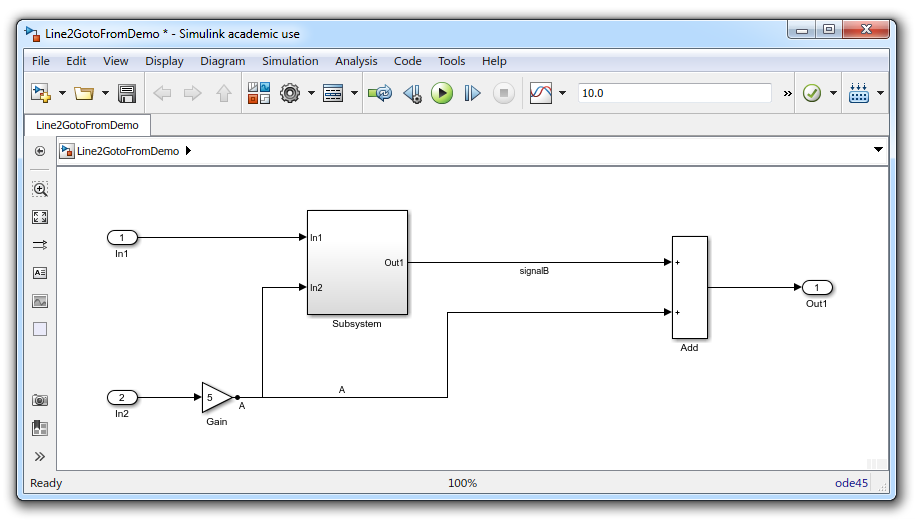
\includegraphics[width=\textwidth]{../figs/Demo2}
	\caption{Resulting model after \cmd{Goto/Froms to Line} transformation on \block{A} \goto/\from blocks.}
	\label{FIG:demo2}
\end{figure}

\begin{figure}
	\centering
	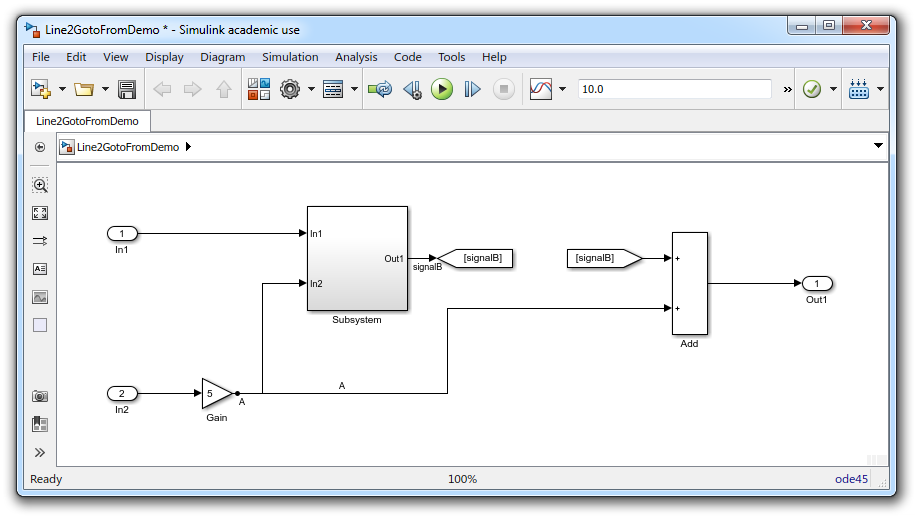
\includegraphics[width=\textwidth]{../figs/Demo3}
	\caption{Resulting model after \cmd{Line to Goto/Froms} transformation on \keyword{signalB}.}
	\label{FIG:demo3}
\end{figure}

%%%%%%%%%%%%%%%%%%%%%%%%%%%%%%%%%%%%%%%%%%%%%%%%%%%%%%%%%%%%%%%%%%%
% Matlab Commands
%%%%%%%%%%%%%%%%%%%%%%%%%%%%%%%%%%%%%%%%%%%%%%%%%%%%%%%%%%%%%%%%%%%
\section{Matlab Commands}

The tool can also be used via the \Matlab command line, with the following functions.

%---------------------------------------
% Command 1
%---------------------------------------
\begin{center}
	\begin{tabular}{| >{\columncolor[gray]{0.9}}l | p{8.5cm} |} \hline
		Function 		& \func{1}~ \\ \hline
		Syntax			& \func{1}~(\args{address, blocks}) \\ \hline
		Description		& Converts selected local \goto/\from block connections into signal lines.\\ \hline
		Inputs		& \args{address}:  Path of where the \goto/\from blocks reside in the model. \newline
								\args{blocks}:  Cell array of \goto/\from block pathnames or handles to convert. \\ \hline	
		Outputs			& N/A \\ \hline
	\end{tabular}
\end{center}

\paragraph{Example:} The following command transforms the \goto/\from blocks with tag \keyword{A}, named \block{From0}, into a signal line connection in model \demoName. The resulting model is shown as Figure~\ref{FIG:demo2}.

\begin{center}
	\cmd{\func{1}~(`\demoName', \{`test2/From0'\})}
\end{center}

%---------------------------------------
% Command 2
%---------------------------------------
\begin{center}
	\begin{tabular}{| >{\columncolor[gray]{0.9}}l | p{8.5cm} |} \hline
		Function 		& \func{2}~ \\ \hline
		Syntax			& \func{2}~(\args{address, line, tag}) \\ \hline
		Description		& Converts a signal line into a \goto/\from connection.\\ \hline
		Inputs	& \args{address}: Path of where the signal line resides in the model. \newline
						  \args{line}:  Handle of the signal line to convert. \newline
						  \args{tag}:  Valid variable name\footnote{\url{https://www.mathworks.com/help/matlab/ref/isvarname.html}} char array, to be used as the \goto/\from tag. \\ \hline
		Outputs			& N/A \\ \hline
	\end{tabular}
\end{center}

\paragraph{Example:} The following command transforms the signal line named \keyword{signalB}, with line handle given as variable \keyword{lh}, into a \goto/\from block connection in model \demoName. The resulting model is shown as Figure~\ref{FIG:demo3}.

\begin{center}
	\cmd{\func{2}~(`\demoName', lh, `signalB')}
\end{center}

\textit{\textbf{Note:} Included with this tool are two functions, \cmd{gcl} and \cmd{gcls}, which get the current line handle(s) for one or more lines, respectively. They are provided to assist with the command line operation of this tool.}

\end{document}